% ---
% titre: 9P - Nombres relatifs
% theme: NO
% chapitre: Nombres relatifs
% sous_chapitre:
% niveau: [9e]
% type: PLANIF
% tags: [c-nombres-relatifs,c-priorite-operations,c-operations,c-addition,c-division,c-multiplication,c-soustraction]
% source: latex 
% ---

\header{Nombres relatifs - Objectifs}

\def\arraystretch{1.2}
\begin{tabularx}{\linewidth}{|>{\centering\arraybackslash}p{3cm}|>{\centering\arraybackslash}p{3cm}|X|}
\hline
\cellcolor{themeNO!30} Livre & \cellcolor{themeNO!30} Fiches & \cellcolor{themeNO!30} \hfill Aide-mémoire\hfill\null\\
\hline
\multirow{2}{*}{pp. 44-57}&\multirow{2}{*}{pp. 39-55}&Généralités: pp. 24-26\\
&&Nombres relatifs: pp. 31-34\\
\hline
\end{tabularx}
\def\arraystretch{1}


\def\arraystretch{1.6}
\begin{tabularx}{\textwidth}{|>{\raggedright\arraybackslash}X|>{\raggedright\arraybackslash}X|}
\hline
\cellcolor{themeNO!30}Compétences visées & \cellcolor{themeNO!30}Utilité dans la vie de tous les jours \\
\hline
Mobiliser les savoirs, savoir-faire et savoir être pour résoudre des problèmes en lien avec les nombres relatifs.
&\vspace{-1em}
\begin{itemize}[leftmargin=*, itemsep=2pt, topsep=0pt, partopsep=0pt, parsep=0pt, label=$\triangleright$]
    \item Évaluer la température
    \item Se repérer entre les étages d'un bâtiment
    \item Évaluer les prix, les dépenses, le salaire
\end{itemize} \\
\hline

Développer des stratégies de recherche afin de résoudre des problèmes.
&\vspace{-1em}
\begin{itemize}[leftmargin=*, itemsep=2pt, topsep=0pt, label=$\triangleright$]
    \item Découper un projet en sous-tâches
    \item Choisir l'ordre des tâches à effectuer
\end{itemize} \\
\hline

Présenter sa démarche de façon claire (explications, grandeur cherchée, unités, calculs, réponse).
&\vspace{-1em}
\begin{itemize}[leftmargin=*, itemsep=2pt, topsep=0pt, label=$\triangleright$]
    \item Collaborer avec d'autres personnes
    \item Expliciter sa compréhension d'un sujet
    \item Argumenter
\end{itemize} \\
\hline

Développer des stratégies d'apprentissage pour s'approprier puis mobiliser les savoirs et savoir-faire.
&\vspace{-1em}
\begin{itemize}[leftmargin=*, itemsep=2pt, topsep=0pt, label=$\triangleright$]
    \item Apprendre une nouvelle activité %(art, sport, \ldots)
    \item S'adapter à un nouvel environnement %(travail, voyage, \ldots)
    \item Se former en autonomie %(tutoriel, lecture, \ldots)
\end{itemize} \\
\hline

Vérifier sa solution ou au moins sa plausibilité.
&\vspace{-1em}
\begin{itemize}[leftmargin=*, itemsep=2pt, topsep=0pt, label=$\triangleright$]
    \item S'autocritiquer
    \item Évaluer la qualité de son travail
\end{itemize} \\
\hline
\end{tabularx}
\def\arraystretch{1}


\vfill
\begin{astuce}{Ce que je dois déjà savoir}
\begin{itemize}[leftmargin=*, itemsep=2pt, topsep=2pt, label=$\triangleright$]
    \item Maîtriser les livrets jusqu'à 12 \hfill (NO 9.1)
    \item Effectuer les quatre opérations avec des nombres naturels et décimaux \hfill (NO 9.1)
    \item Connaître les priorités des opérations (\textcolor{themeNO}{PEMDAS}) \hfill (NO 9.1)
\end{itemize}
\end{astuce}

\newpage
%---------------
\def\arraystretch{1.6}
\begin{tabularx}{\textwidth}{|>{\raggedright\arraybackslash}p{5.2cm}|>{\raggedright\arraybackslash}X|>{\centering\arraybackslash}p{0.8cm}|>{\centering\arraybackslash}p{0.8cm}|>{\centering\arraybackslash}p{0.8cm}|}
\hline
\rowcolor{themeNO!30}\multicolumn{2}{|l|}{Objectifs} &\multicolumn{3}{c|}{Auto-évaluation} \\
\rowcolor{themeNO!30}\multicolumn{2}{|l|}{} & \Sadey[1.5]& \Neutrey[1.5] & \Smiley[1.5]  \\\hline

\multirow{2}{=}{Connaître et utiliser les différentes écritures d'un même nombre relatif}
& Connaître le vocabulaire lié aux nombres relatifs~: ordre croissant et décroissant, nombre positif et négatif, nombres opposés & & & \\
\cline{2-5}
& Déterminer la distance à zéro (valeur absolue) d'un nombre relatif & & & \\
\hline

\multirow{4}{=}{Comparer, approximer, encadrer et représenter sur une droite des nombres relatifs}
& Graduer une droite des nombres et y placer des nombres relatifs & & & \\
\cline{2-5}
& Calculer l'écart entre deux nombres relatifs & & & \\
\cline{2-5}
& Comparer deux nombres relatifs à l'aide des signes $<$, $>$, $=$ & & & \\
\cline{2-5}
& Classer des nombres relatifs par ordre croissant ou décroissant à l'aide de la droite numérique & & & \\
\hline

\multirow{5}{=}{Utiliser des procédures de calcul réfléchi ou de calcul mental avec des nombres relatifs de $-100$ à $+100$~: $+$, $-$, $\cdot$, $:$}
& Simplifier l'écriture d'une somme ou d'une différence de nombres relatifs (signes et parenthèses inutiles) & & & \\
\cline{2-5}
& Additionner des nombres relatifs à l'aide des règles de calcul ou de déplacements sur la droite des nombres & & & \\
\cline{2-5}
& Soustraire un nombre relatif en additionnant son opposé & & & \\
\cline{2-5}
& Déterminer le signe d'un produit ou d'un quotient de nombres relatifs & & & \\
\cline{2-5}
& Multiplier et diviser des nombres relatifs & & & \\
\hline
\end{tabularx}
\def\arraystretch{1}

\vfill
\begin{astuce}{Mon bilan}
Ce que je dois encore travailler~:\\[2pt]
\noindent\makebox[\linewidth]{\dotfill}\\[2pt]
\noindent\makebox[\linewidth]{\dotfill}\\[7pt]
Ce que je peux faire pour progresser~:\\[2pt]
\noindent\makebox[\linewidth]{\dotfill}\\[2pt]
\noindent\makebox[\linewidth]{\dotfill}
\end{astuce}

%------------------------------------------------
\newpage
\header{Nombres relatifs - Feuille de route}

\newcommand{\rref}[1]{\textcolor{themeColor}{#1}}

% Case à cocher
\newcommand{\case}{\raisebox{-0.1ex}{\Large$\square$}}

% Marqueurs obligatoire / facultatif (forme, pas seulement couleur)
\newcommand{\oblig}{\tikz[baseline=-0.5ex]{\fill[themeColor] (0,0) circle (0.09);}}
\newcommand{\faclt}{\tikz[baseline=-0.5ex]{\draw[gray!70,line width=0.6pt] (0,0) circle (0.09);}}

 \vfill
\begin{tikzpicture}[
circ/.style={circle, fill=themeColor, text=white, font=\bfseries\Large, minimum size=11mm, inner sep=0pt},
 box/.style={rectangle, draw=themeColor!35!white, rounded corners=2pt, fill=themeColor!8!white, inner sep=3mm, text width=14.7cm, align=left, anchor=north west}]

% ---------- Étape 1 ----------
\node[circ, anchor=north] (c1) at (0,0) {1};
\node[box] (b1) at ($(c1.north)+(1.2cm,0)$) {%
\textbf{\large Découverte des nombres relatifs}\\[4pt]
{\small\begin{tabularx}{10cm}{cXp{3cm}p{1cm}}
\case & \rref{NO 106} & Livre, p.\,47 & \oblig \\
\case & \rref{NO 105} & Livre, p.\,46 & \oblig \\
\case & \rref{NO 111} & Fiche, p.\,40 & \oblig \\
\end{tabularx}}
};

% ---------- Étape 2 ----------
\coordinate (y2) at ($(b1.south west)+(0,-3mm)$);
\node[circ, anchor=north] (c2) at (c1 |- y2) {2};
\node[box] (b2) at (y2) {%
\textbf{\large Comparaison de nombres relatifs}\\[4pt]
{\small\begin{tabularx}{10cm}{cXp{3cm}p{1cm}}
\case & \rref{NO 107} & Livre, p.\,47 & \oblig \\
\case & \rref{NO 108} & Livre, p.\,47 & \oblig \\
\end{tabularx}}
};

% ---------- Étape 3 ----------
\coordinate (y3) at ($(b2.south west)+(0,-3mm)$);
\node[circ, anchor=north] (c3) at (c1 |- y3) {3};
\node[box] (b3) at (y3) {%
\textbf{\large Addition et soustraction de nombres relatifs}\\[4pt]
{\small\begin{tabularx}{10cm}{cXp{3cm}p{1cm}}
\case & \rref{NO 117}      & Livre, p.\,49 & \oblig \\
\case & \rref{NO 118}      & Livre, p.\,49 & \oblig \\
\case & \rref{NO 123}      & Livre, p.\,51 & \oblig \\
\case & \rref{NO 124}      & Livre, p.\,51 & \oblig \\
\case & \rref{Problème 11} & VLM, p.\,9    & \oblig \\
\case & \rref{Problème 17} & VLM, p.\,13   & \oblig \\
\end{tabularx}}
};

% ---------- Étape 4 ----------
\coordinate (y4) at ($(b3.south west)+(0,-3mm)$);
\node[circ, anchor=north] (c4) at (c1 |- y4) {4};
\node[box] (b4) at (y4) {%
\textbf{\large Multiplication et division de nombres relatifs}\\[4pt]
{\small\begin{tabularx}{10cm}{cXp{3cm}p{1cm}}
\case & \rref{NO 142}      & Livre, p.\,54 & \oblig \\
\case & \rref{NO 143}      & Livre, p.\,55 & \oblig \\
\case & \rref{NO 146}      & Livre, p.\,55 & \oblig \\
\case & \rref{NO 147}      & Livre, p.\,55 & \oblig \\
\case & \rref{Problème 12} & VLM, p.\,9    & \oblig \\
\end{tabularx}}
};

% ---------- Étape 5 ----------
\coordinate (y5) at ($(b4.south west)+(0,-3mm)$);
\node[circ, anchor=north] (c5) at (c1 |- y5) {5};
\node[box] (b5) at (y5) {%
\textbf{\large Quatre opérations sur les nombres relatifs}\\[4pt]
{\small\begin{tabularx}{10cm}{cXp{3cm}p{1cm}}
\case & \rref{Problème 13 A. à D.} & VLM, p.\,10 & \oblig \\
\case & Problème 19                       & VLM, p.\,14 & \faclt \\
\case & Problème 13 E. à P.               & VLM, p.\,10 & \faclt \\
\case & Problème 14 A*. à P*.             & VLM, p.\,11 & \faclt \\
\end{tabularx}}
};

% ---------- Étape 6 ----------
\coordinate (y6) at ($(b5.south west)+(0,-3mm)$);
\node[circ, anchor=north] (c6) at (c1 |- y6) {6};
\node[box] (b6) at (y6) {%
\textbf{\large Exercices \guillemotleft\,Défi\,\guillemotright}\\[4pt]
{\small\begin{tabularx}{10cm}{cXp{3cm}p{1cm}}
\case & NO 137 & Fiche, p.\,48 & \faclt \\
\case & NO 151 & Fiche, p.\,51 & \faclt \\
\case & NO 152 & Fiche, p.\,52 & \faclt \\
\case & NO 156 & Fiche, p.\,53 & \faclt \\
\case & NO 158 & Livre, p.\,57 & \faclt \\
\end{tabularx}}
};

% ---------- Ligne de parcours (derrière les cercles) ----------
\begin{pgfonlayer}{background}
\draw[themeColor, line width=2pt] (c1) -- (c2) -- (c3) -- (c4) -- (c5) -- (c6);
\end{pgfonlayer}

\end{tikzpicture}

 \vfill
\begin{center}
\small \case~à faire \qquad \oblig~\rref{obligatoire} \qquad \faclt~facultatif (consolidation / pour aller plus loin)
\end{center}
\vspace{1em}

%------------------------------------------------
\newpage
\header{Nombres relatifs - Théorie}

\subsection*{1. Les nombres relatifs}

\begin{regle}{Définition}
Les \textcolor{themeNO}{nombres relatifs} sont les nombres entiers positifs (précédés du signe $+$), négatifs (précédés du signe $-$) et zéro. Leur ensemble se note $\mathbb{Z}$.
\end{regle}

\vspace{10pt}
\begin{center}
$\mathbb{Z}=\left\{\ldots,\,-3,\,-2,\,-1,\,0,\,+1,\,+2,\,+3,\,\ldots\right\}$
\end{center}

\vspace{10pt}
On peut représenter les nombres relatifs sur une \textcolor{themeNO}{droite numérique}.

\vspace{20pt}
\begin{center}
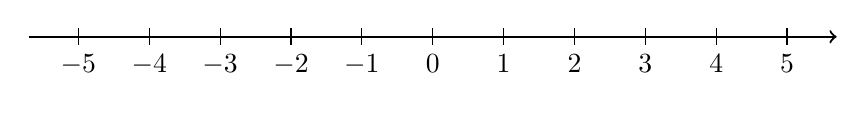
\begin{tikzpicture}[scale=0.9]
\draw[->, thick] (-5.7,0) -- (5.7,0);
\foreach \x in {-5,...,+5}
  \draw (\x,0.12) -- (\x,-0.12) node[below] {$\x$};
\end{tikzpicture}
\end{center}

\vfill
\subsection*{2. Nombres opposés et valeur absolue}

\begin{regle}{Définition}
Deux nombres relatifs sont \textcolor{themeNO}{opposés} s'ils sont à la même distance de zéro, de part et d'autre de zéro sur la droite numérique.
\end{regle}

\begin{center}
$+5$ et $-5$ sont opposés, car ils sont tous deux à $5$ unités de zéro.
\end{center}

\vspace{20pt}
\begin{regle}{Définition}
La \textcolor{themeNO}{valeur absolue} d'un nombre relatif est sa valeur sans prendre en compte le signe. Elle se note entre deux barres verticales $\lvert\ \ \ \rvert$.
\end{regle}

\begin{center}
$\lvert -7\rvert=7$ \quad\quad et \quad\quad $\lvert +5\rvert=5$
\end{center}

\vspace{20pt}
La valeur absolue s'appelle aussi la \textcolor{themeNO}{distance à zéro}, puisqu'elle correspond à la distance entre le nombre et zéro sur la droite numérique.

\newpage
\subsection*{3. Graduer une droite des nombres}

\begin{astuce}{Marche à suivre}
\begin{enumerate}[leftmargin=*, itemsep=2pt, topsep=2pt]
    \item Tracer une droite avec une flèche vers la droite.
    \item Placer le \textcolor{themeNO}{zéro}.
    \item Choisir une \textcolor{themeNO}{unité} (de 1 en 1, de 2 en 2, de 10 en 10, \ldots) et reporter toujours la même distance entre deux graduations.
    \item Placer les nombres positifs à droite de zéro et les nombres négatifs à gauche.
\end{enumerate}
\end{astuce}

\vspace{10pt}
Exemple 1: 

\begin{center}
\begin{tikzpicture}[scale=0.9]
\draw[->, thick] (-5.7,0) -- (5.7,0);
\foreach \x in {-4,...,4}{
  \pgfmathtruncatemacro{\v}{\x*10}
  \draw (\x*1.3,0.12) -- (\x*1.3,-0.12) node[below] {$\v$};
}
\foreach \x in {-3.5,-2.5,...,3.5}
  \draw (\x*1.3,0.06) -- (\x*1.3,-0.06);
\foreach \p/\l in {-3.9/-30, -0.65/-5, 3.25/25}{
  \fill[themeNO] (\p,0) circle (0.1);
  \node[above=5pt, themeNO] at (\p,0) {$\l$};
}
\end{tikzpicture}\\[6pt]
Ici, l'unité est de 10~: entre deux graduations, il y a 10. Les nombres $-5$ et $25$ sont placés au milieu entre deux graduations.
\end{center}

\vspace{10pt}
Exemple 2 :

\begin{center}
\begin{tikzpicture}[scale=0.9]
\draw[->, thick] (-5.7,0) -- (5.7,0);
\foreach \x in {-4,...,4}{
  \pgfmathtruncatemacro{\v}{\x*2}
  \draw (\x*1.3,0.12) -- (\x*1.3,-0.12) node[below] {$\v$};
}
\foreach \x in {-3.5,-2.5,...,3.5}
  \draw (\x*1.3,0.06) -- (\x*1.3,-0.06);
\foreach \p/\l in {-4.55/-7, -1.3/-2, 3.25/5}{
  \fill[themeNO] (\p,0) circle (0.1);
  \node[above=5pt, themeNO] at (\p,0) {$\l$};
}
\end{tikzpicture}\\[6pt]
Ici, l'unité est de 2~: entre deux graduations, il y a 2. Les nombres $-7$ et $5$ sont placés au milieu entre deux graduations.
\end{center}

\vfill
\subsection*{4. Écart entre deux nombres relatifs}

L'\textcolor{themeNO}{écart} entre deux nombres relatifs est la distance qui les sépare sur la droite numérique. Pour le calculer, on utilise la distance à zéro (valeur absolue) de chacun d'eux.

\vspace{10pt}
\def\arraystretch{2}
\begin{tabularx}{\linewidth}{|>{\raggedright\arraybackslash}X|>{\raggedright\arraybackslash}X|}
\hline
Si les deux nombres ont \textcolor{themeNO}{le même signe}, on \textcolor{themeNO}{soustrait} leurs valeurs absolues. & Si les deux nombres ont \textcolor{themeNO}{des signes différents}, on \textcolor{themeNO}{additionne} leurs valeurs absolues.\\\hline
Écart entre $-8$ et $-3$~:\newline $8-3=5$ & Écart entre $-3$ et $5$~:\newline $3+5=8$\\\hline
\end{tabularx}
\def\arraystretch{1}

\newpage
\subsection*{5. Comparer des nombres relatifs}

\begin{regle}{Définition}
\textcolor{themeNO}{Comparer} deux nombres relatifs, c'est déterminer lequel est le plus petit. Sur la droite numérique, le plus petit des deux est celui qui est situé le plus à gauche.
\end{regle}

\begin{center}
\begin{tikzpicture}[scale=0.9]
\draw[->, thick] (-6.7,0) -- (6.7,0);
\foreach \x in {-6,...,6}
  \draw (\x,0.12) -- (\x,-0.12) node[below] {$\x$};
\foreach \x in {-5,-2,3}
  \fill[themeNO] (\x,0) circle (0.1);
\draw[themeNO, <-] (-5.5,0.7) -- (-0.5,0.7) node[midway, above] {\small plus petit};
\draw[themeNO, ->] (0.5,0.7) -- (5.5,0.7) node[midway, above] {\small plus grand};
\end{tikzpicture}\\[6pt]
$-5$ est à gauche de $-2$, donc $-5<-2$. \quad $-2$ est à gauche de $3$, donc $-2<3$.
\end{center}

\vspace{20pt}
\begin{astuce}{Les signes de comparaison}
$<$ se lit \og\,plus petit que\,\fg~: $-5<-2$\\[2pt]
$>$ se lit \og\,plus grand que\,\fg~: $3>-4$\\[2pt]
$=$ se lit \og\,égal à\,\fg~: $\lvert -7\rvert=7$\\[2pt]
La pointe du signe $<$ ou $>$ est toujours tournée vers le \textcolor{themeNO}{plus petit} nombre.
\end{astuce}

\vfill
\begin{regle}{Propriété}
Un nombre \textcolor{themeNO}{négatif} est toujours plus petit que zéro et que tout nombre positif.
\end{regle}

\begin{center}
$-13<0$ \quad\quad et \quad\quad $-13<4$
\end{center}

\vfill
\begin{regle}{Propriété}
Si deux nombres sont négatifs, le plus petit des deux est celui dont la \textcolor{themeNO}{valeur absolue} est la plus grande.
\end{regle}

\begin{center}
$\lvert -20\rvert=20>\lvert -12\rvert=12$ \quad donc \quad $-20<-12$
\end{center}

\vspace{20pt}
\begin{astuce}{Pour s'en souvenir}
Pense à un thermomètre. Quand il fait $-20\,^\circ$C, il fait plus froid que lorsqu'il fait $-12\,^\circ$C. Ainsi, $-20\,^\circ$C est une température plus basse que $-12\,^\circ$C.
\end{astuce}

\newpage
\subsection*{6. Ordre croissant et décroissant}

\begin{regle}{Définition}
Ranger des nombres dans l'ordre \textcolor{themeNO}{croissant}, c'est les ranger du plus petit au plus grand.\\[2pt]
Ranger des nombres dans l'ordre \textcolor{themeNO}{décroissant}, c'est les ranger du plus grand au plus petit.
\end{regle}

\begin{center}
$-7<-2<0<3$ \quad est un rangement dans l'ordre croissant.\\[2pt]
$3>0>-2>-7$ \quad est un rangement dans l'ordre décroissant.
\end{center}

\vfill
\subsection*{7. La règle des signes}

Lorsque deux signes se suivent, on les remplace par un seul signe.

\def\arraystretch{1.6}
\begin{tabularx}{\linewidth}{|c|c|>{\centering\arraybackslash}X|}
\hline
\textbf{Les deux signes} & \textbf{Donnent} & \textbf{Exemple}\\\hline
$+$ et $+$ & $+$ & $3+(+5)=3+5=8$\\\hline
$-$ et $-$ & $+$ & $3-(-5)=3+5=8$\\\hline
$+$ et $-$ & $-$ & $3+(-5)=3-5=-2$\\\hline
$-$ et $+$ & $-$ & $3-(+5)=3-5=-2$\\\hline
\end{tabularx}
\def\arraystretch{1}

\begin{astuce}{À retenir}
Deux signes \textcolor{themeNO}{identiques} donnent un $+$.\\[2pt]
Deux signes \textcolor{themeNO}{différents} donnent un $-$.
\end{astuce}

\vspace{6pt}
Cette règle sert aussi pour la multiplication et la division (voir section 11).

\vfill
\subsection*{8. Addition}

\def\arraystretch{2}
\begin{tabularx}{\linewidth}{|>{\centering\arraybackslash}p{2cm}|>{\raggedright\arraybackslash}X|>{\raggedright\arraybackslash}p{3.6cm}|}
\hline
\textbf{Signes identiques} & On \textcolor{themeNO}{additionne} les valeurs absolues. \newline On \textcolor{themeNO}{conserve} le signe commun. & $(+3)+(+9)=(+12)$\newline $(-11)+(-7)=(-18)$\\\hline
\textbf{Signes différents} & On \textcolor{themeNO}{soustrait} la plus petite valeur absolue de la plus grande. \newline On \textcolor{themeNO}{utilise} le signe du nombre qui a la plus grande valeur absolue. & $(-26)+(+7)=(-19)$\newline $(+4)+(-31)=(-27)$\\\hline
\end{tabularx}
\def\arraystretch{1}

\newpage
\subsection*{9. Soustraction}

\begin{astuce}{À retenir}
Pour soustraire un nombre relatif, on additionne son \textcolor{themeNO}{opposé}.
\end{astuce}

\begin{center}
$(+13)-(+12)=(+13)+(-12)=(+1)$\\[3pt]
$(+25)-(-37)=(+25)+(+37)=(+62)$\\[3pt]
$(-33)-(-29)=(-33)+(+29)=(-4)$
\end{center}

\vfill
\subsection*{10. Calculer une suite d'additions et de soustractions}

\begin{astuce}{Marche à suivre}

\vspace{-6pt}
\textbf{Simplifier l'écriture}
\begin{enumerate}[leftmargin=*, itemsep=2pt, topsep=2pt]
    \item Supprimer les parenthèses.
    \item Lorsque deux signes se suivent, appliquer la règle des signes.
\end{enumerate}

\vspace{10pt}
\textbf{Calculer}
\begin{enumerate}[resume, leftmargin=*, itemsep=2pt, topsep=2pt]
    \item Repérer les nombres positifs (point au-dessus) et les nombres négatifs (point au-dessous).
    \item Additionner tous les nombres positifs.
    \item Additionner tous les nombres négatifs : le résultat est précédé du signe $-$.
    \item Soustraire la plus petite valeur absolue de la plus grande.
    \item Utiliser le signe de la plus grande valeur absolue.
\end{enumerate}
\end{astuce}

\vspace{15pt}
Exemple :

\vspace{-25pt}\begin{align*}
&(-8)+(-9)-(+5)+(+4)+(-7)-(-6)-(-2)+(+10)-(+7)\\[-2pt]
\intertext{On supprime les parenthèses et on applique la règle des signes~:}
&=-8-9-5+4-7+6+2+10-7\\[-2pt]
\intertext{On repère les nombres positifs (un point au-dessus) et les nombres négatifs (un point au-dessous)~:}
&=-\underset{\bullet}{8}-\underset{\bullet}{9}-\underset{\bullet}{5}\mathbin{\textcolor{themeNO}{+}}\textcolor{themeNO}{\overset{\bullet}{4}}-\underset{\bullet}{7}\mathbin{\textcolor{themeNO}{+}}\textcolor{themeNO}{\overset{\bullet}{6}}\mathbin{\textcolor{themeNO}{+}}\textcolor{themeNO}{\overset{\bullet}{2}}\mathbin{\textcolor{themeNO}{+}}\textcolor{themeNO}{\overset{\bullet}{10}}-\underset{\bullet}{7}\\[-2pt]
\intertext{On additionne les positifs ($4+6+2+10=22$) et les négatifs ($8+9+5+7+7=36$)~:}
&=22-36\\[-2pt]
\intertext{Les signes sont différents : on soustrait $36-22=14$ et on garde le signe de 36 ($-$)~:}
&=-14
\end{align*}

\newpage
\subsection*{11. Multiplication et division}

Pour multiplier ou diviser deux nombres relatifs :
\begin{enumerate}[leftmargin=*, itemsep=2pt, topsep=2pt]
    \item on multiplie (ou on divise) les \textcolor{themeNO}{valeurs absolues} ;
    \item on applique la \textcolor{themeNO}{règle des signes}.
\end{enumerate}

\begin{center}
\def\arraystretch{1.4}
\begin{tabular}{|c|c|c|}
\hline
\textbf{Signe du premier nombre} & \textbf{Signe du deuxième nombre} & \textbf{Signe du résultat}\\\hline
$+$ & $+$ & $+$\\\hline
$+$ & $-$ & $-$\\\hline
$-$ & $+$ & $-$\\\hline
$-$ & $-$ & $+$\\\hline
\end{tabular}
\def\arraystretch{1}
\end{center}

Deux signes \textcolor{themeNO}{identiques} donnent un $+$ et deux signes \textcolor{themeNO}{différents} donnent un $-$.

\vspace{20pt}
\def\arraystretch{1.6}
\begin{tabularx}{\linewidth}{|>{\raggedright\arraybackslash}p{3cm}|>{\centering\arraybackslash}X|>{\centering\arraybackslash}X|}
\hline
\textbf{Multiplication} & $(-5)\cdot(-10)=(+50)$\newline $(+7)\cdot(-2)=(-14)$ & $(-6)\cdot(+4)=(-24)$\newline $(+3)\cdot(+9)=(+27)$\\\hline
\textbf{Division} & $(+16):(+4)=(+4)$\newline $(+36):(-12)=(-3)$ & $(-10):(+5)=(-2)$\newline $(-30):(-6)=(+5)$\\\hline
\end{tabularx}
\def\arraystretch{1}

\vfill
\subsection*{12. Plusieurs multiplications et divisions}

\begin{astuce}{Règle des signes}
S'il y a plusieurs multiplications et/ou divisions à la suite, on compte le nombre de signes \og$-$\fg.\\[2pt]
Si ce nombre est \textcolor{themeNO}{pair}, le résultat est \textcolor{themeNO}{positif}.\\[2pt]
Si ce nombre est \textcolor{themeNO}{impair}, le résultat est \textcolor{themeNO}{négatif}.
\end{astuce}

\vspace{20pt}
\def\arraystretch{1.6}
\begin{tabularx}{\linewidth}{|>{\centering\arraybackslash}X|>{\raggedright\arraybackslash}X|}
\hline
$(-2)\cdot 3:2\cdot(-5):(-1)=-15$ & Il y a 3 signes \og$-$\fg. 3 est impair. Le résultat est négatif.\\\hline
$(-3)\cdot 7\cdot(-4)=84$ & Il y a 2 signes \og$-$\fg. 2 est pair. Le résultat est positif.\\\hline
\end{tabularx}
\def\arraystretch{1}

\newpage
\subsection*{13. Calculs avec les quatre opérations}

Les priorités des opérations (\textcolor{themeNO}{PEMDAS}) s'appliquent aussi avec les nombres relatifs.

\begin{astuce}{Priorité des opérations}
1. Parenthèses \quad 2. Exposants \quad 3. Multiplications et divisions \quad 4. Additions et soustractions\\[2pt]
À chaque étape, on calcule de gauche à droite.
\end{astuce}

\vspace{20pt}
Exemple 1 :

\begin{align*}
(-3)\cdot(+4)-(-10):(+2)&=&&\text{On effectue d'abord $\cdot$ et $:$ (règle des signes).}\\
-12-(-5)&=&&\text{On simplifie les signes.}\\
-12+5&=&&\text{Signes différents : $12-5=7$, signe de 12.}\\
-7&&&
\end{align*}

Exemple 2 :

\begin{align*}
5-2\cdot(-3+1)&=&&\text{On calcule d'abord la parenthèse.}\\
5-2\cdot(-2)&=&&\text{On effectue la multiplication.}\\
5-(-4)&=&&\text{On simplifie les signes.}\\
5+4&=&&\text{On additionne.}\\
9&&&
\end{align*}

Exemple 3 :

\begin{align*}
(+7)-(-2)\cdot(+3)&=&&\text{On effectue d'abord la multiplication.}\\
(+7)-(-6)&=&&\text{On simplifie les signes et on enlève le $+$ du premier nombre.}\\
7+6&=&&\text{On additionne.}\\
13&&&
\end{align*}

%------------------------------------------------
\newpage
\header{Nombres relatifs - Lexique}

\newtcolorbox{terme}{%
  enhanced, sharp corners, boxrule=0pt, colback=themeColor!6!white,
  colframe=themeColor!6!white,
  borderline west={2.2pt}{0pt}{themeColor},
  left=3mm, right=2mm, top=2mm, bottom=2mm,
}
 
 %\vfill
\begin{tcbraster}[raster columns=2, raster equal height, raster valign=top,raster column skip=2mm, raster row skip=2mm]
\begin{terme}
\textbf{\large Comparer}\\[2pt]
{\small Déterminer lequel de deux nombres est le plus petit (ou s'ils sont égaux).}
\end{terme}
\begin{terme}
\textbf{\large Distance à zéro}\\[2pt]
{\small Distance entre un nombre et zéro sur la droite numérique. C'est un autre nom pour la valeur absolue.}
\end{terme}
\begin{terme}
\textbf{\large Droite numérique}\\[2pt]
{\small Droite graduée sur laquelle on représente les nombres. Ils augmentent de gauche à droite.}
\end{terme}
\begin{terme}
\textbf{\large Écart}\\[2pt]
{\small Distance qui sépare deux nombres sur la droite numérique.}
\end{terme}
\begin{terme}
\textbf{\large Ensemble $\mathbb{Z}$}\\[2pt]
{\small Ensemble de tous les nombres entiers relatifs~: $\ldots,\,-2,\,-1,\,0,\,1,\,2,\,\ldots$}
\end{terme}
\begin{terme}
\textbf{\large Nombre négatif}\\[2pt]
{\small Nombre plus petit que zéro, précédé du signe $-$.}
\end{terme}
\begin{terme}
\textbf{\large Nombre positif}\\[2pt]
{\small Nombre plus grand que zéro, précédé du signe $+$ (souvent omis).}
\end{terme}
\begin{terme}
\textbf{\large Nombre relatif}\\[2pt]
{\small Nombre entier précédé d'un signe $+$ ou $-$, ou zéro.}
\end{terme}
\begin{terme}
\textbf{\large Nombres opposés}\\[2pt]
{\small Deux nombres à la même distance de zéro, mais de signes différents (par exemple $+5$ et $-5$).}
\end{terme}
\begin{terme}
\textbf{\large Ordre croissant}\\[2pt]
{\small Rangement des nombres du plus petit au plus grand.}
\end{terme}
\begin{terme}
\textbf{\large Ordre décroissant}\\[2pt]
{\small Rangement des nombres du plus grand au plus petit.}
\end{terme}
\begin{terme}
\textbf{\large Règle des signes}\\[2pt]
{\small Deux signes identiques donnent un $+$, deux signes différents donnent un $-$.}
\end{terme}
\begin{terme}
\textbf{\large Signe}\\[2pt]
{\small Symbole $+$ ou $-$ placé devant un nombre.}
\end{terme}
\begin{terme}
\textbf{\large Valeur absolue}\\[2pt]
{\small Valeur d'un nombre sans son signe. Elle se note entre deux barres verticales~: $\lvert -7\rvert=7$.}
\end{terme}
\end{tcbraster}